\documentclass{standalone}
\usepackage{tikz}
\usetikzlibrary{arrows}
\begin{document}
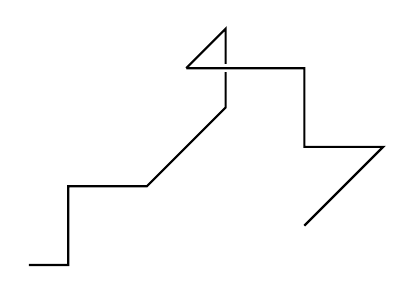
\begin{tikzpicture}[scale=(0.5)]
\draw[thick] (0,0) -- (1,0) -- (1,2) -- (3,2) -- (5,4) -- (5,6) -- (4,5);
\draw[white, line width=1mm] (4.5,5) -- (5.5,5);
\draw[thick] (4,5) -- (7,5) -- (7,3) -- (9,3) -- (7,1);
\end{tikzpicture}
\hspace{1cm}
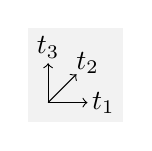
\begin{tikzpicture}[scale=(0.5)]
\fill[black!5!] (-.5,-.5) -- (1.9,-.5) -- (1.9,1.9) -- (-.5,1.9);
\draw[->] (0,0) -- (1,0);
\draw[->] (0,0) -- (0,1);
\draw[->] (0,0) -- (.72,.72);
\node at (1.4,0) {$t_1$};
\node at (1,1) {$t_2$};
\node at (0,1.4) {$t_3$};
\end{tikzpicture}
\hspace{1cm}
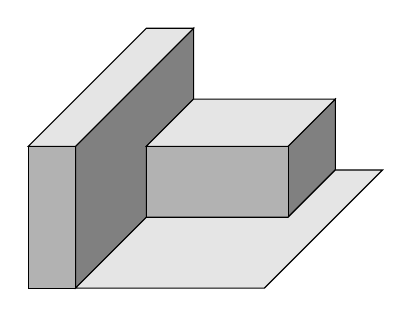
\begin{tikzpicture}[scale=(0.3)]
\filldraw[fill=black!50!, draw=black] (-3,-3) -- (-3,3) -- (2,8) -- (2,5) -- (0,3) -- (0,0) -- cycle;
\filldraw[fill=black!50!, draw=black] (6,0) -- (6,3) -- (8,5) -- (8,2) -- cycle;

\filldraw[fill=black!30!, draw=black] (0,3) -- (6,3) -- (6,0) -- (0,0) -- cycle;
\filldraw[fill=black!30!, draw=black] (-3,-3) -- (-5,-3) -- (-5,3) -- (-3,3) -- cycle;

\filldraw[fill=black!10!, draw=black] (-3,-3) -- (5,-3) -- (10,2) -- (8,2) -- (6,0) -- (0,0) -- cycle;
\filldraw[fill=black!10!, draw=black] (0,8) -- (-5,3) -- (-3,3) -- (2,8) -- cycle;
\filldraw[fill=black!10!, draw=black] (0,3) -- (2,5) -- (8,5) -- (6,3) -- cycle;
\end{tikzpicture}
\end{document}